\documentclass{beamer}
\usetheme{Madrid}
\usepackage{wrapfig}
\title{THE LOOP OF ARTIFICIAL INTELLIGENCE: AN INTRODUCTION}
\author{Rajasekhar}
\institute[Asian Institute of Technology]
{\inst{}Department of Information and Communication Technology\\Asian Institute of Technology, Thailand}
\date{December 2017}
\begin{document}
\begin{frame}
  \titlepage
\end{frame}
\begin{frame}{Overview}
 \begin{figure}
     \centering
     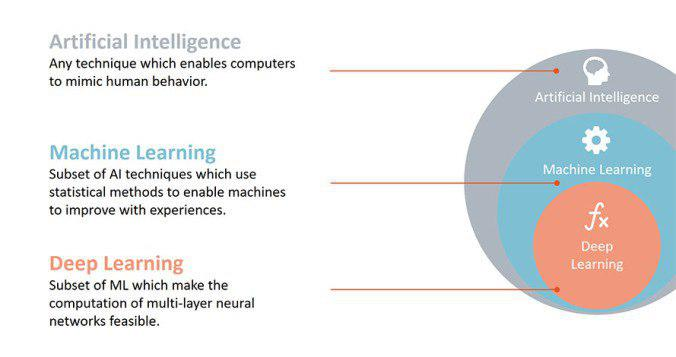
\includegraphics[width=4in\textwidth]{fig/ai-ml.jpg}
     \caption{AI and its subsets}
     \label{fig:AI and its subsets}
 \end{figure}
\end{frame}
\begin{frame}{Machine Learning (ML)}
  \begin{itemize}
  \item As a subset of AI, it is mainly to understand the structure of data and fit that data into models which are understandable and utilized by people. 
  \item Traditional computing and ML-Algorithmic computing.
  \item Popular areas include \textbf{Facial recognition}, \textbf{Optical character recognition (OCR)}.
  \item Famous algorithmic approaches such as K-Nearest Neighbour (K-NN), Decision trees, Support vector machines (SVMs), and Deep learning.
  \end{itemize}
\end{frame}
\begin{frame}{ML- Methods}
    \begin{itemize}
    \item The classification is based on the learning perspectives. The main two classifications are \textbf{Supervised learning} and \textbf{Unsupervised learning}.
    \item In \textbf{supervised learning}, the labeled data-sets are given as input to the computer. Here, the algorithmic computation is to learn by comparing the data-sets to the learned ones. 
    \item As a result in supervised learning, it helps to build the model with the historic data the likely future events.
    \item In \textbf{unsupervised learning}, the data-sets are unlabeled. The algorithmic computation is fed to draw the common points among the input data. 
    \end{itemize}
\end{frame}
\begin{frame}{ML- Methods (cont...)}{Supervised Learning}
\begin{figure}
    \centering
    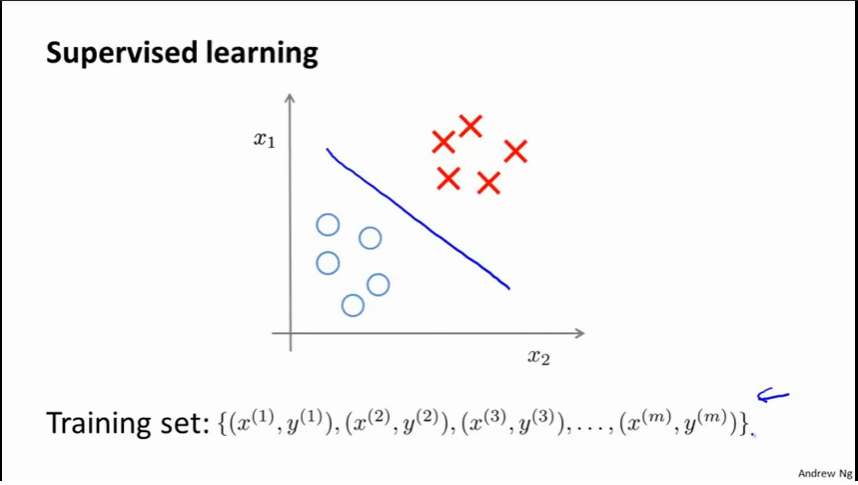
\includegraphics[width=.9\textwidth]{fig/supv.png}
    \caption{Supervised learning}
    \label{fig:Supervised learning}
\end{figure}
\end{frame}
\begin{frame}{ML- Methods (cont...)}{Unsupervised Learning}
    \begin{figure}
        \centering
        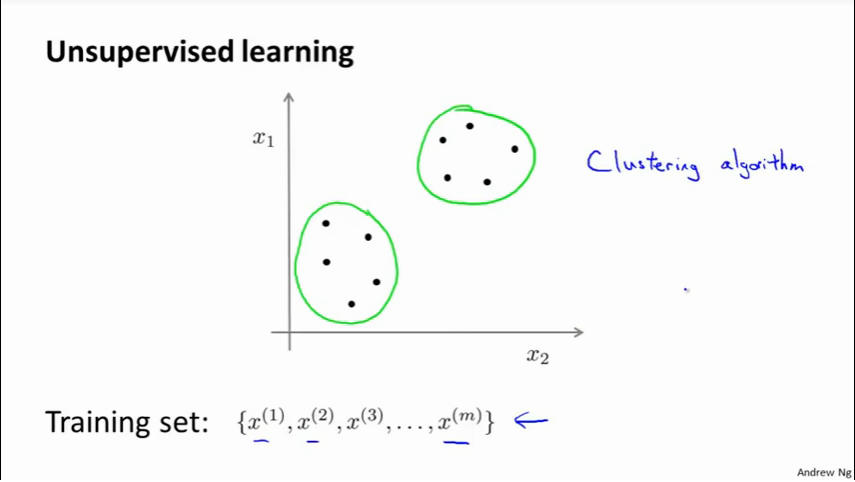
\includegraphics[width=.9\textwidth]{fig/uns.png}
        \caption{Unsupervised learning}
        \label{fig:Unsupervised learning}
    \end{figure}
\end{frame}
\begin{frame}{ML- Methods (cont...)}{A few examples}
    \begin{figure}
        \centering
        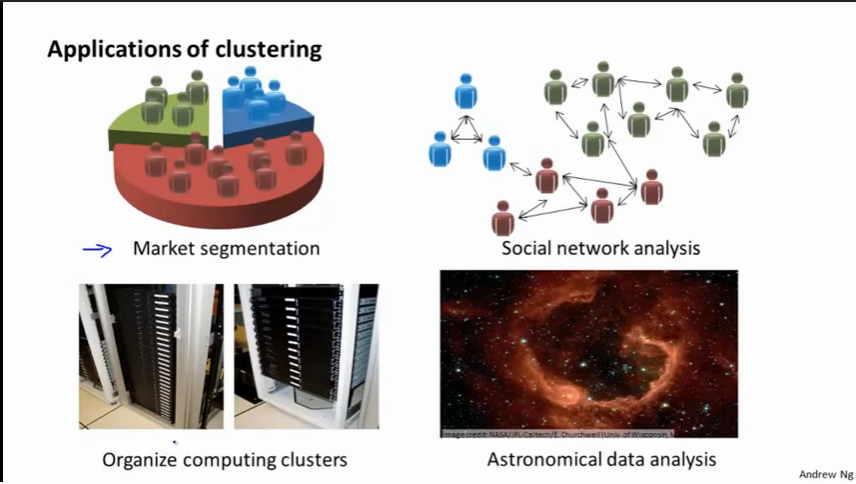
\includegraphics[width=.9\textwidth]{fig/un-app.png}
        \caption{Examples}
        \label{fig:Examples}
    \end{figure}
\end{frame}
\begin{frame}{Finding an Approach}
    \begin{itemize}
        \item \textbf{Correlation} and \textbf{Regression} are the most commonly used statistical techniques for investigating the relationship among the quantitative variables.
        \item Correlation is about the association of two variables which are not either dependent or independent. Regression is the combination of dependent and independent variables.
        \item The popular approaches include K-NN classification, Decision Tree learning, and Deep learning.
    \end{itemize}
\end{frame}
\begin{frame}{K- Nearest Neighbours Classification}
    \item Cluster assignment
    \begin{figure}
        \centering
        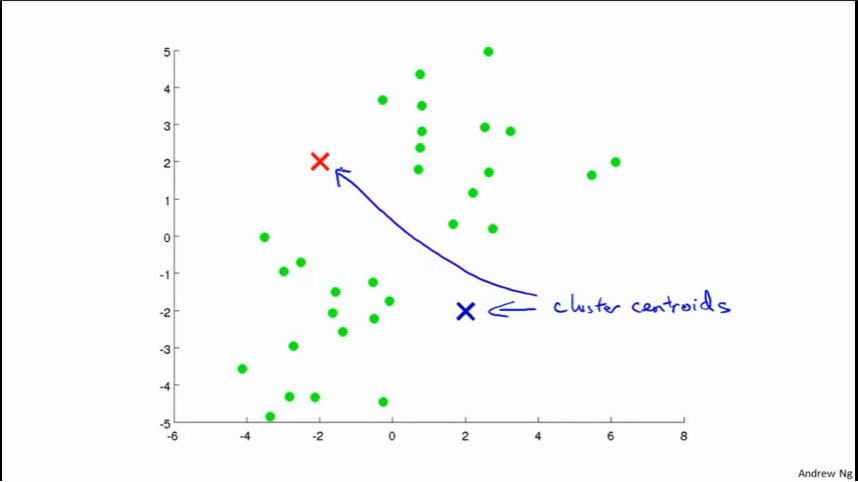
\includegraphics[width=.8\textwidth]{fig/k1.png}
        \caption{Define Clusters}
        \label{fig:Define Clusters}
    \end{figure}
\end{frame}
\begin{frame}{K- NN (cont...)}
    \item Group centroids
    \begin{figure}
        \centering
        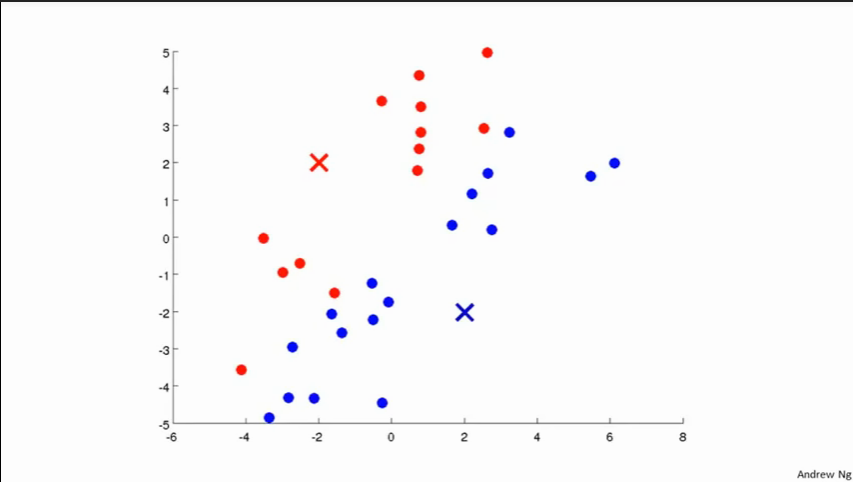
\includegraphics[width=.8\textwidth]{fig/k2.png}
        \caption{Centroids}
        \label{fig:Centroids}
    \end{figure}
\end{frame}
\begin{frame}{K- NN (cont...)}
    \begin{figure}
        \centering
        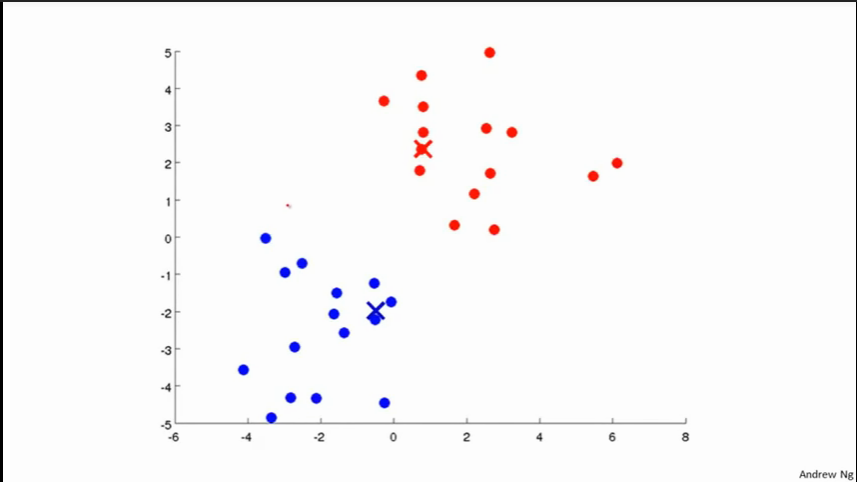
\includegraphics[width=.8\textwidth]{fig/k6.png}
        \caption{Separate clusters}
        \label{fig:Separate clusters}
    \end{figure}
\end{frame}
\begin{frame}{Decision Tree Learning}
    \begin{figure}
        \centering
        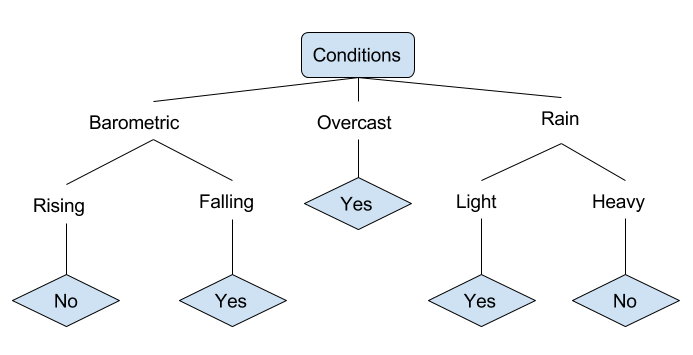
\includegraphics[width=.8\textwidth]{decision-tree-diagram.png}
        \caption{Decision tree}
        \label{fig:Decision tree}
    \end{figure}
\end{frame}
\begin{frame}{Deep Learning}
    \begin{itemize}
        \item Deals the problems with Machine vision (aka Computer vision).
        \item A cascaded layered process approach.
        \item Artificial Neural Networks (ANN) algorithms are more widely used. Others such as SVMs, SIFT, SURF, and SLAM are also used.
        \item Support vector machines used for the clustering problems.
    \end{itemize}
\end{frame}
\begin{frame}{Conclusions}
    \begin{itemize}
    \item Keeping an eye on algorithms, methods, and approaches.
    \item Most used simplified libraries/algorithms in C++ and Python are help full.
    \end{itemize}
\end{frame}
\end{document}